\documentclass[11pt]{beamer}
\usepackage{listings} % Include the listings-package
\usepackage[T1]{fontenc}
\usepackage[utf8]{inputenc}
\usepackage{amsmath}
\usepackage{amssymb, amsfonts,cancel,latexsym }%latexsym}
\usepackage{float}
\usepackage{graphicx}
%\usepackage{epstopdf}
%\usepackage{subfigure}
\usepackage{hyperref}
%\usepackage{blindtext}
%\usepackage{booktabs} % Allows the use of \toprule, 
\usepackage{filecontents}
\usepackage{courier}%% Sets font for listing as Courier.
\usepackage{listings}
\usepackage{listings, xcolor}
\usepackage{epstopdf}

\usepackage{caption}
\DeclareCaptionFont{white}{\color{white}}
\DeclareCaptionFormat{listing}{\colorbox{gray}{\parbox{\textwidth}{#1#2#3}}}
\captionsetup[lstlisting]{format=listing, labelfont=white, textfont=white}
\definecolor{urlColor}{rgb}{0.06, 0.3, 0.57}
\definecolor{linkColor}{rgb}{0.57, 0.0, 0.04}
\definecolor{fileColor}{rgb}{0.0, 0.26, 0.26}
\hypersetup{
    colorlinks=true,
    linkcolor=linkColor,
    filecolor=fileColor,      
    urlcolor=urlColor,
}

\urlstyle{same}
\setbeamercovered{transparent}
%\usetheme{Boadilla}
\usetheme{CambridgeUS}
%\usetheme{Berkeley}
%\usetheme{Warsaw}
%\usetheme{Madrid}

\title[Control Structures]{\bf\Huge Control Structures}
\subtitle{Fundamentals to programming I}

\author[gcondoria]
{
	Graciela Condori Anahua \inst{1}
}
\institute[UNSA]
{
\inst{1}% 
System Engineering School\\
System Engineering and Informatic Department\\
Production and Services Faculty\\
San Agustin National University of Arequipa
}

\date[2020-08-03]{\scriptsize{2020-08-03}}
%\logo{
\includegraphics[width=3.0cm]{img/logo_unsa.jpg}}
\titlegraphic{
\includegraphics[width=3.0cm]{figuras/logo_unsa.jpg}}

\begin{document}

\begin{frame}
\titlepage
\end{frame}

\begin{frame}
\frametitle{Content}
\tableofcontents
\end{frame}

\section{Conditional Structures}
\begin{frame}
\frametitle{Conditional Structures}
\begin{itemize}
\item IF.
\item IF - ELSE.
\item IF - ELSE IF.
\item Nesting.
\item Switch.
\end{itemize}
\end{frame}

\begin{frame}
\frametitle{IF}
\begin{center}
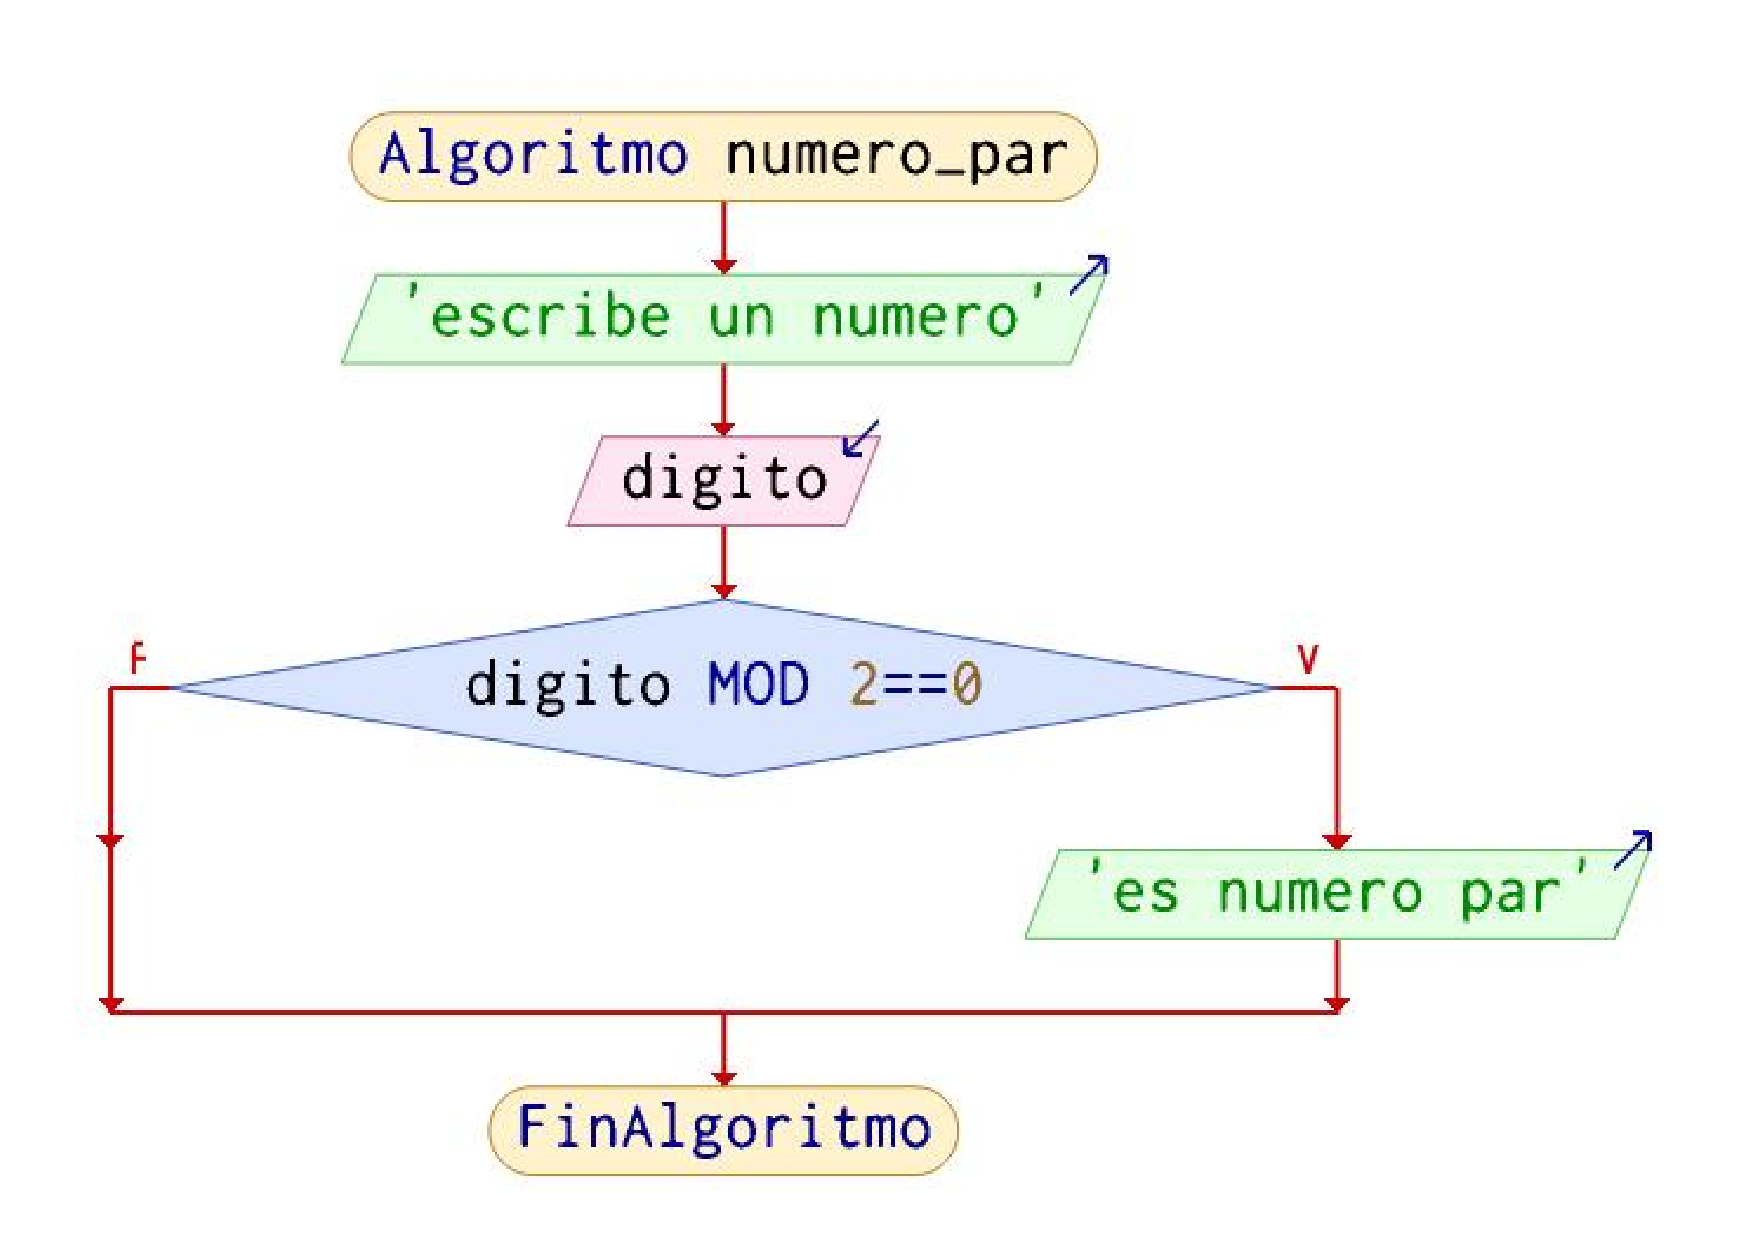
\includegraphics[scale=0.29]{figuras/if..pdf}
\end{center}
\end{frame}

\begin{frame}
\frametitle{IF-ELSE}
\begin{center}
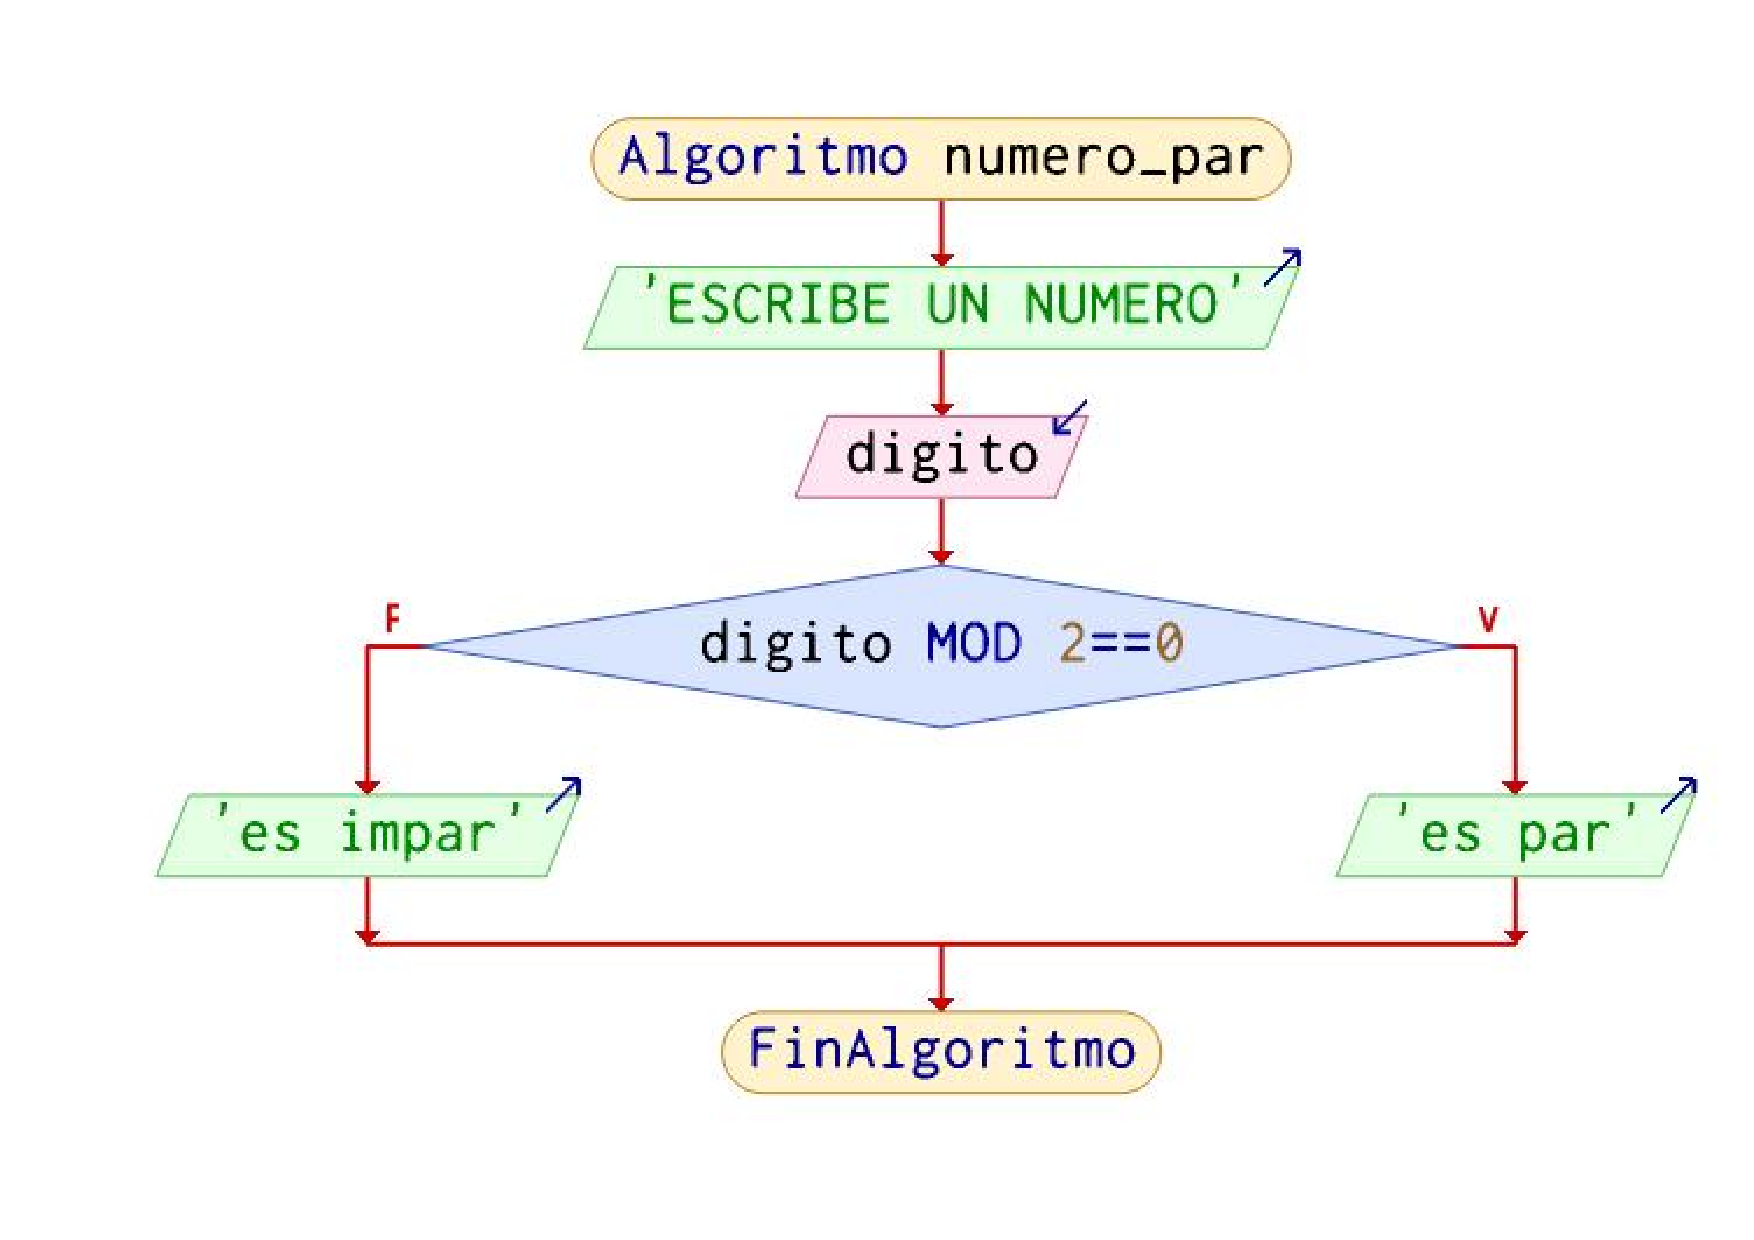
\includegraphics[scale=0.29]{figuras/if.pdf}
\end{center}
\end{frame}

\begin{frame}
\frametitle{IF-ELSE IF}
\begin{center}
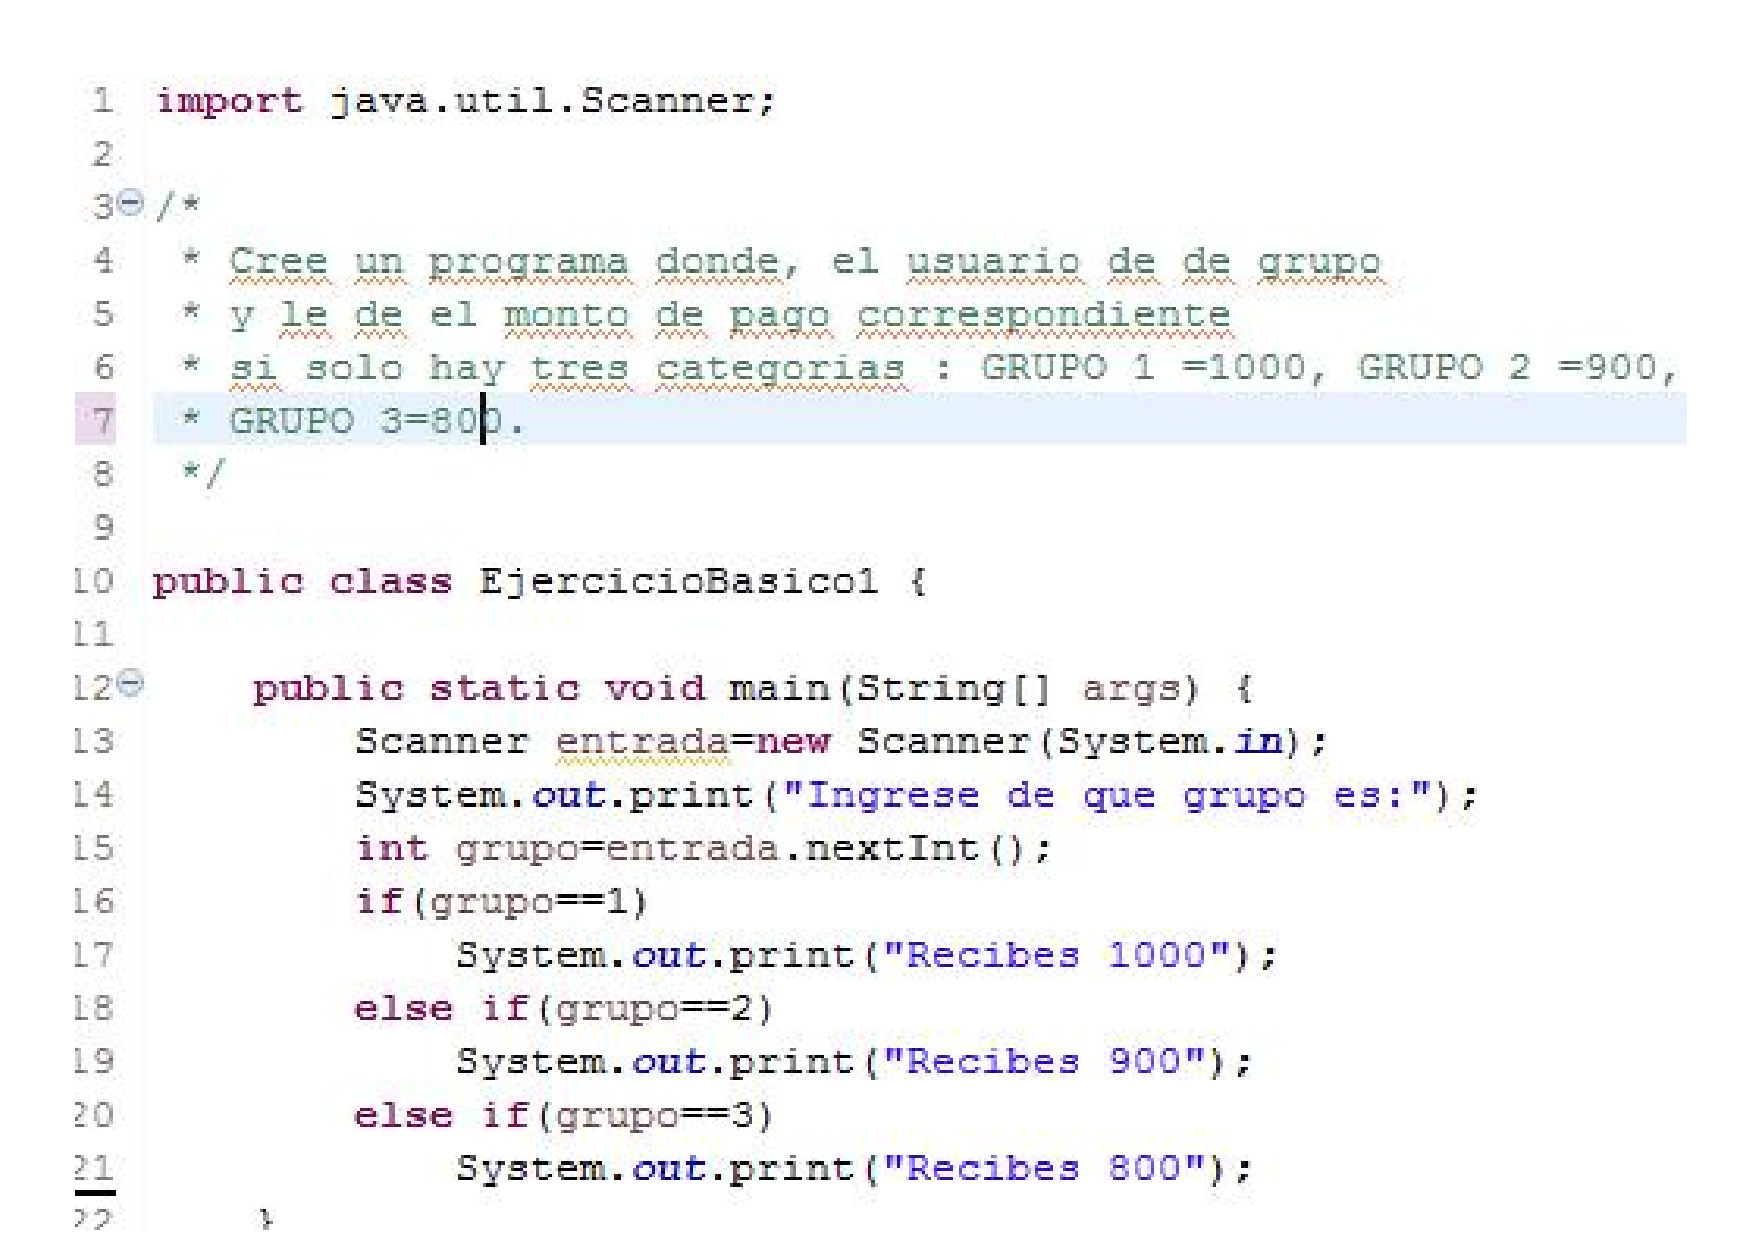
\includegraphics[scale=0.35]{figuras/if_else.pdf}
\end{center}
\end{frame}

\section{Repetitive Structures}
\begin{frame}
\frametitle{Repetitive Structures}
\begin{itemize}
\item WHILE.
\item DO-WHILE.
\item FOR.
\end{itemize}
\end{frame}

\begin{frame}
\frametitle{WHILE}
\begin{center}
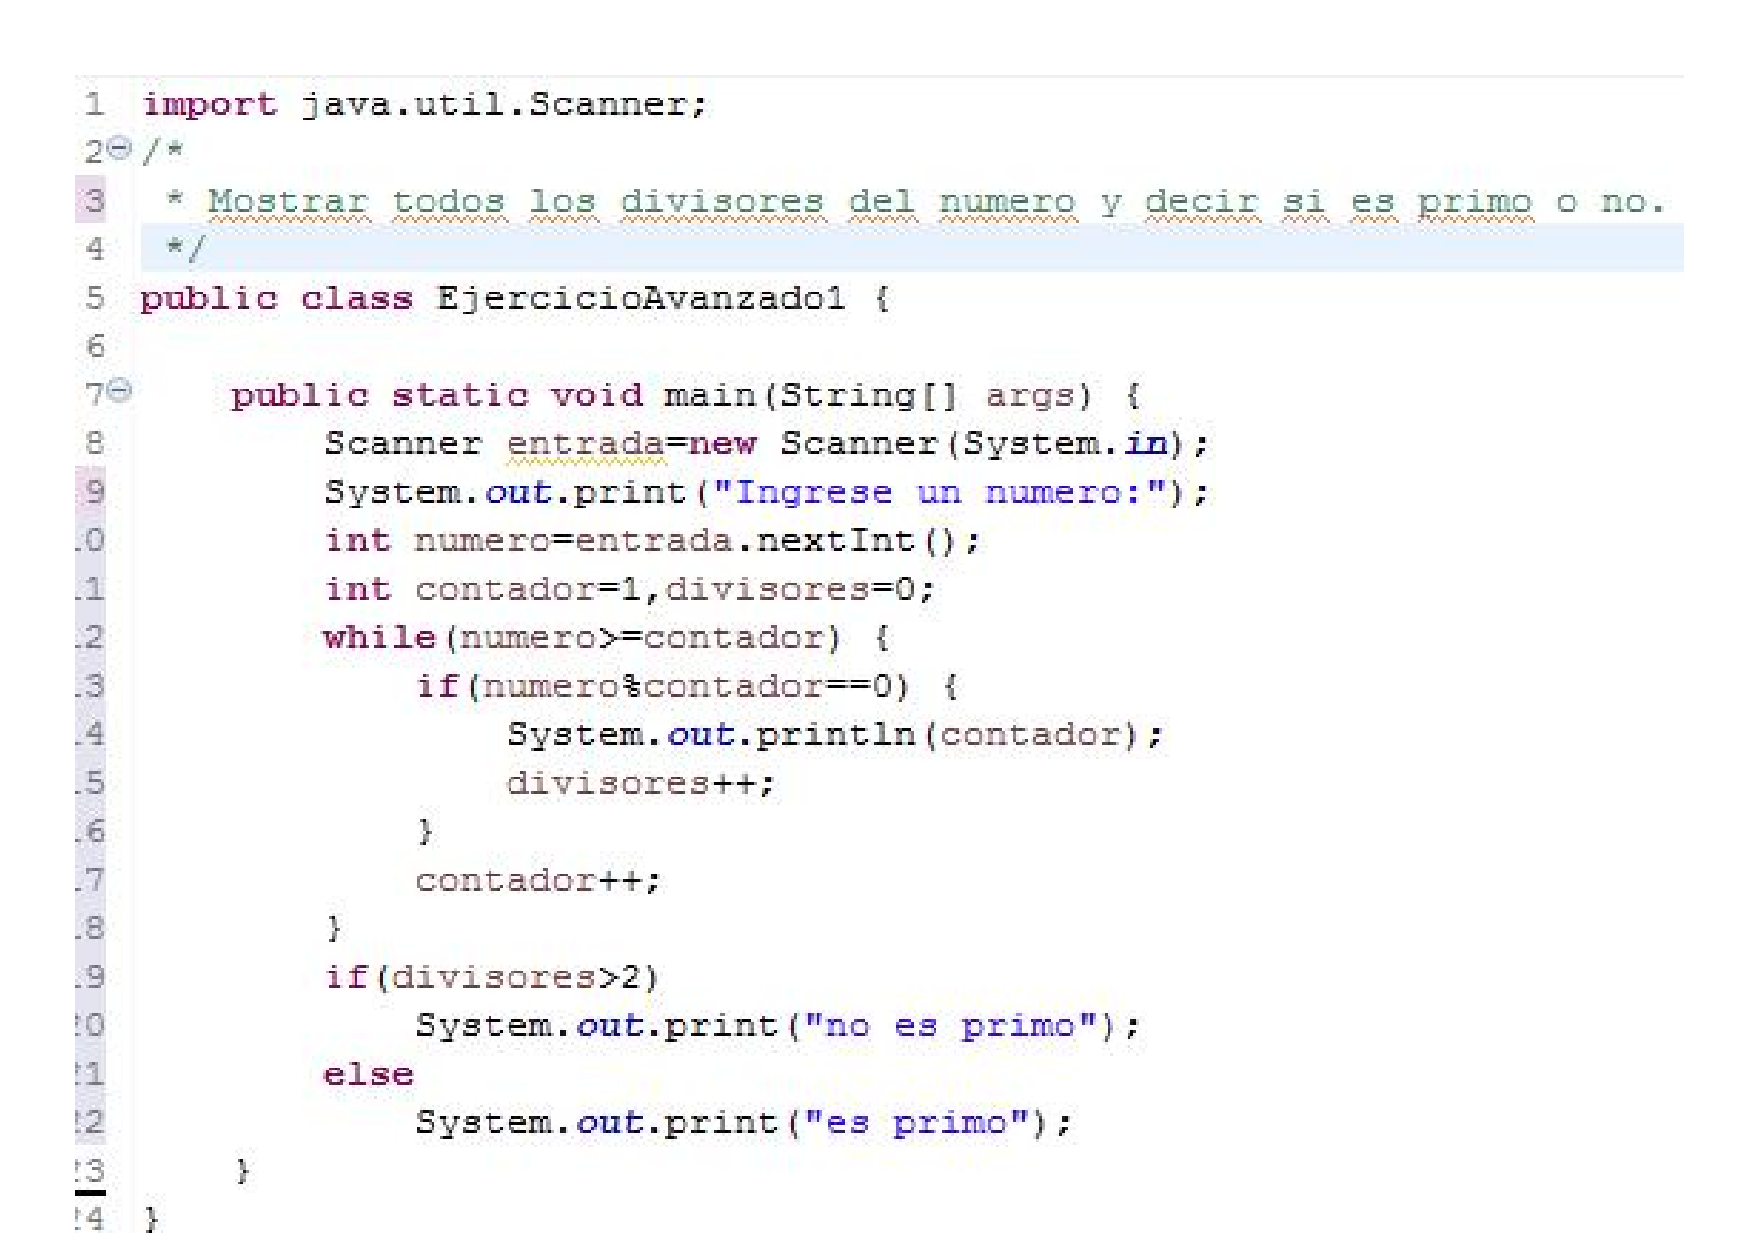
\includegraphics[scale=0.37]{figuras/avanc.pdf}
\end{center}
\end{frame}

\begin{frame}
\frametitle{DO-WHILE}
\begin{center}
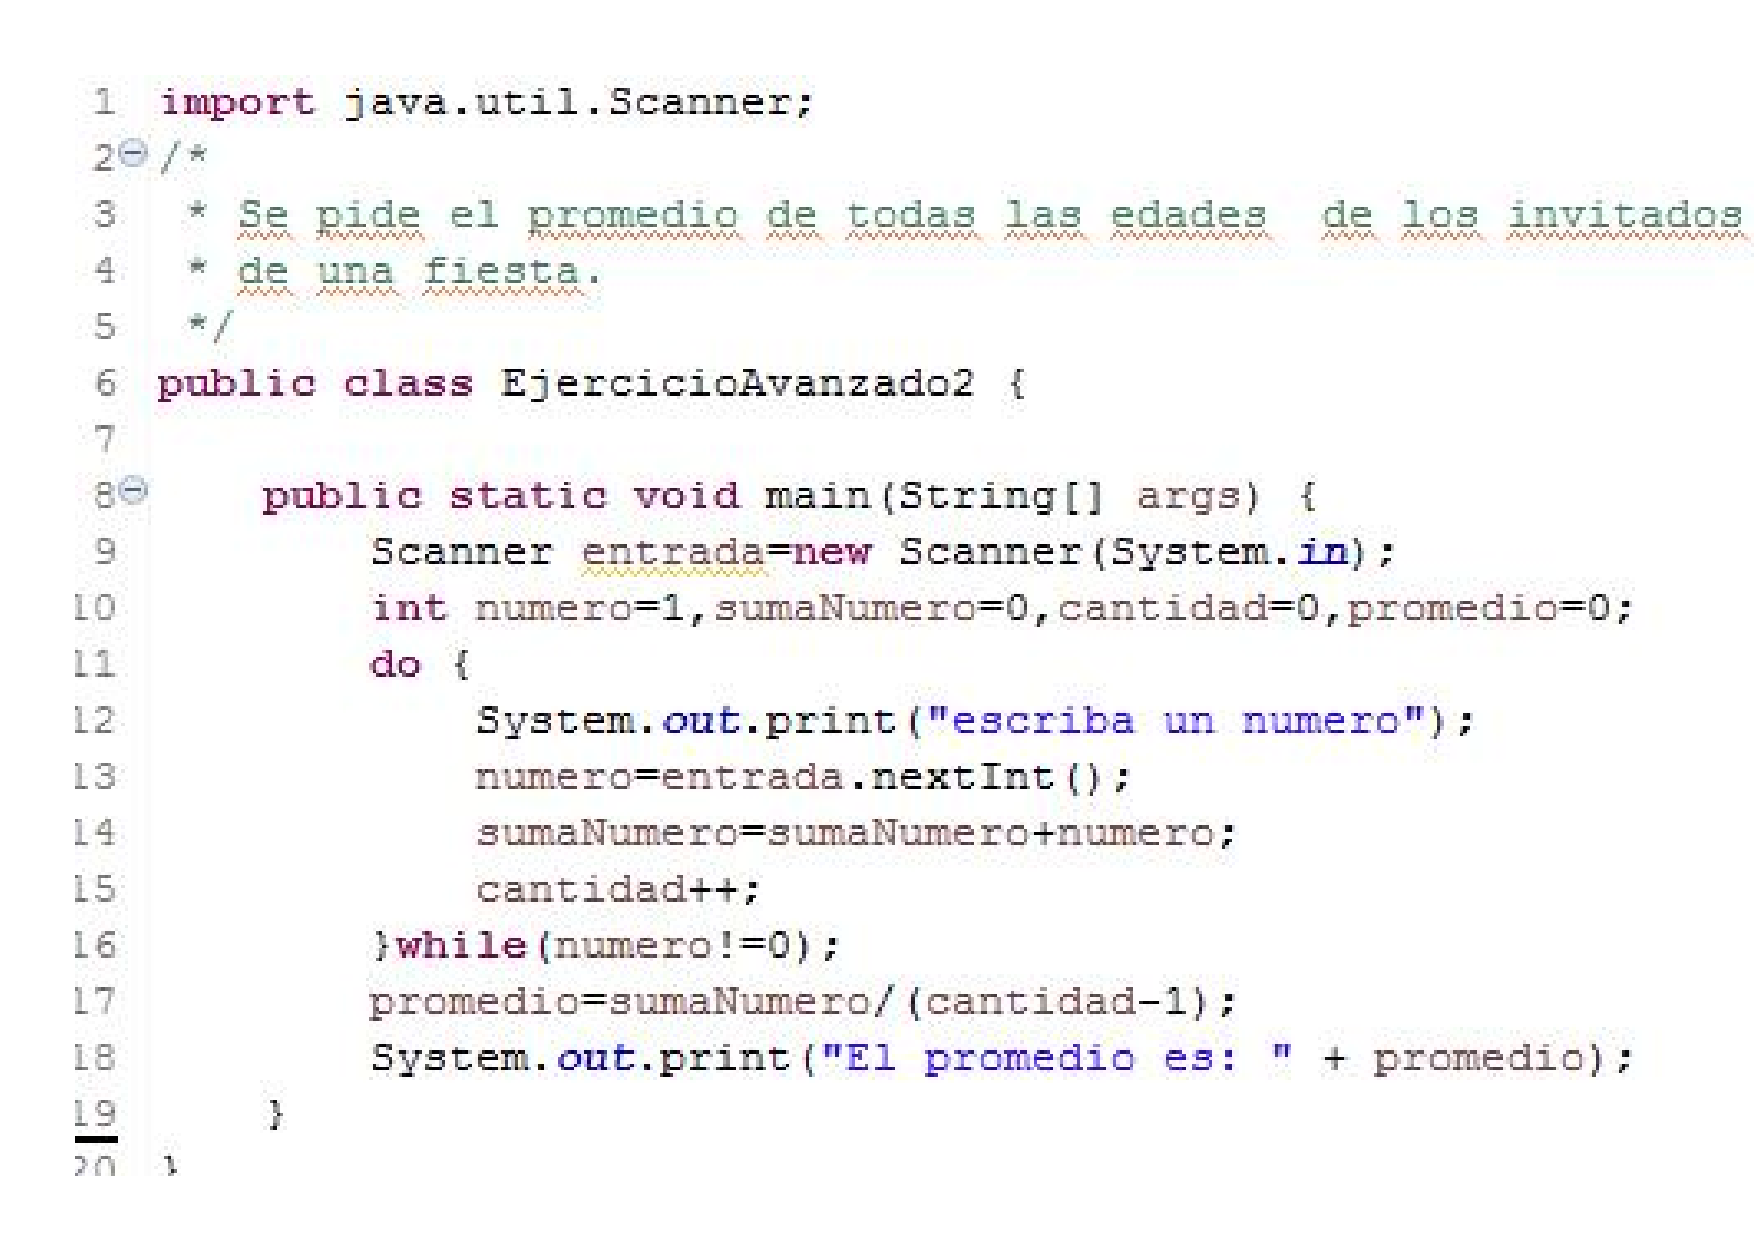
\includegraphics[scale=0.37]{figuras/do_.pdf}
\end{center}
\end{frame}

\begin{frame}
\frametitle{FOR}
\begin{center}
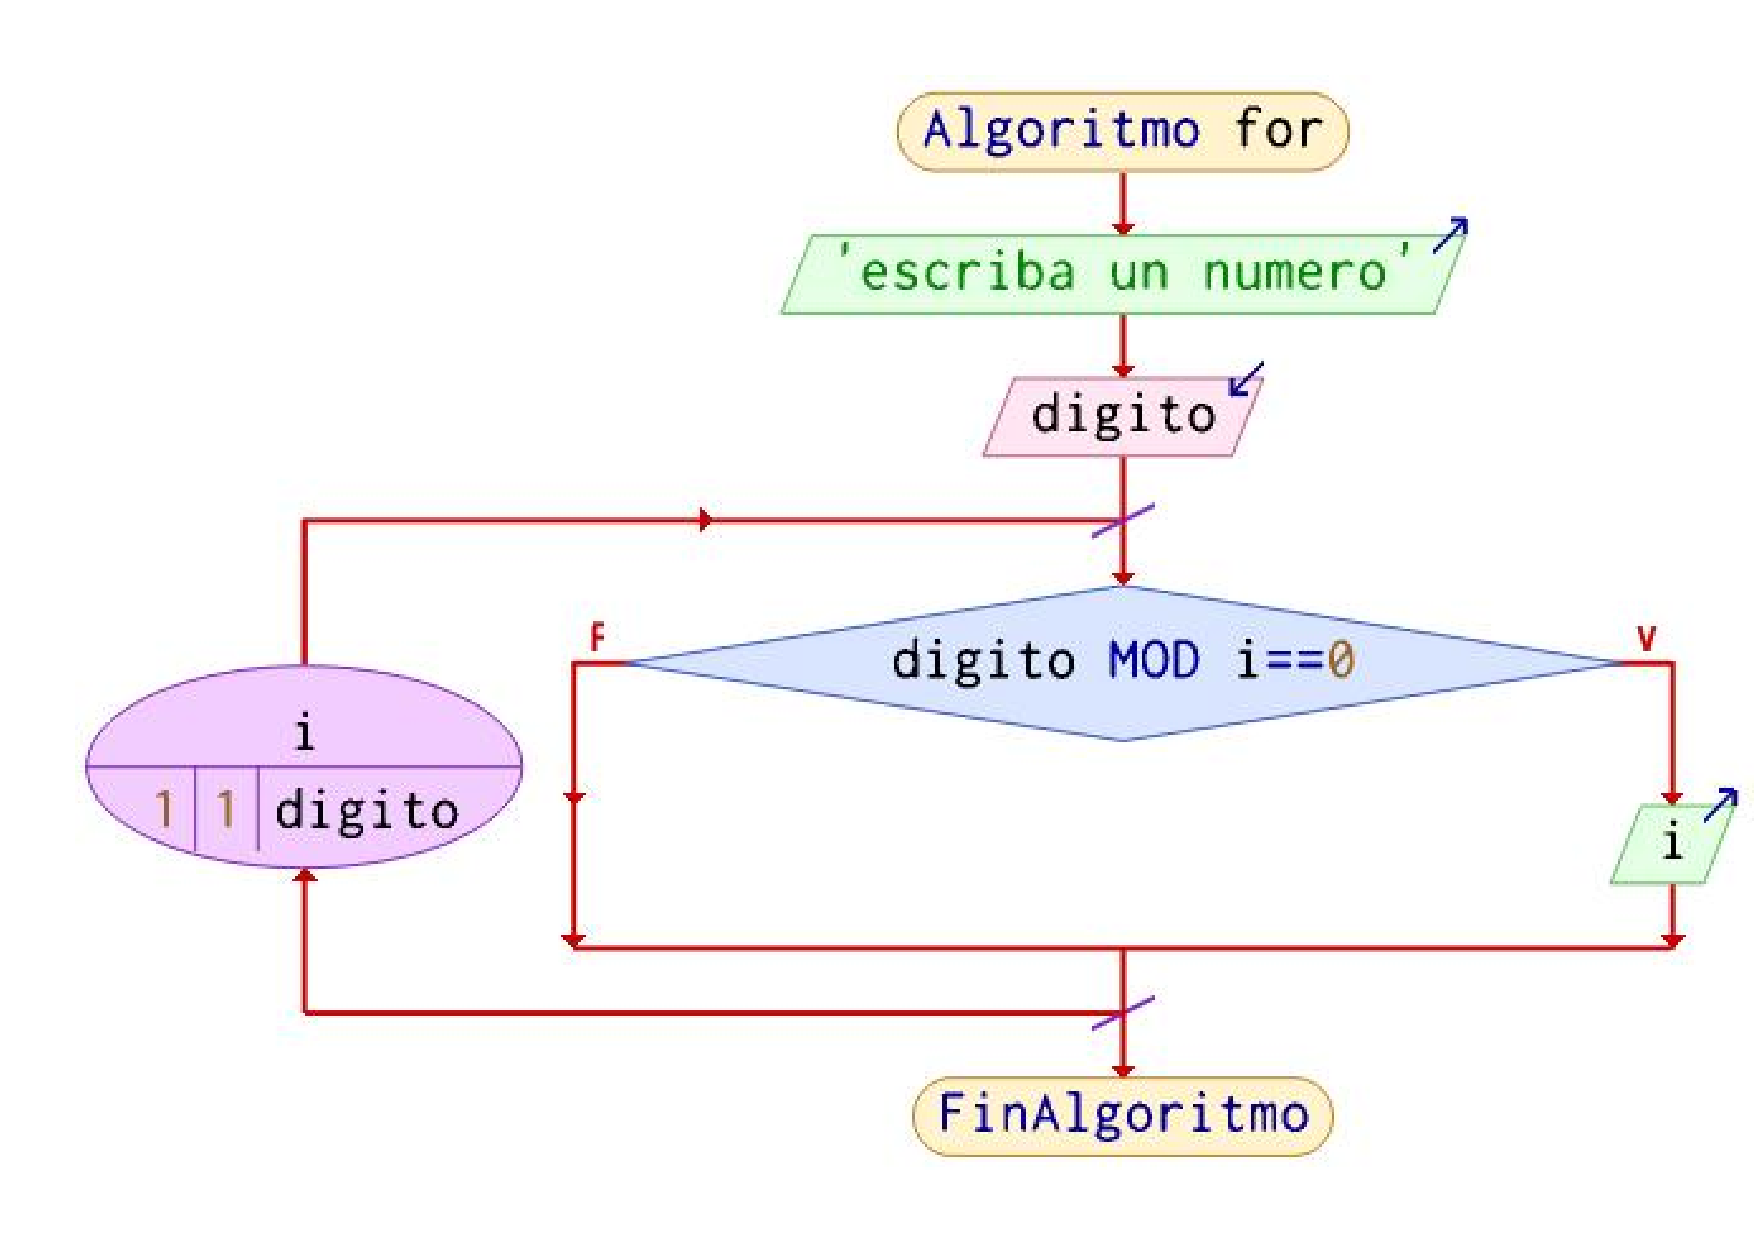
\includegraphics[scale=0.29]{figuras/for.pdf}
\end{center}
\end{frame}

\section{References}
%References frame
\begin{frame}
\frametitle{References - Web pages}
\begin{itemize}
\item \url{https://github.com/rescobedoq/java-00-programming-introduction/blob/master/latex/java-00-programming-introduction.tex}
\item \url{https://elvex.ugr.es/decsai/java/}
\item \url{https://www.oracle.com/java/technologies/javase/javase-jdk8-downloads.html}
\item \url{https://www.eclipse.org/downloads/packages/release/2020-06/r/eclipse-ide-enterprise-java-developers}
\item \url{http://pseint.sourceforge.net/}
\item \url{https://ruidera.uclm.es/xmlui/bitstream/handle/10578/43/programacion_en_C.pdf?sequence=1&isAllowed=y}
\item \url{https://www.pearsoneducacion.net/Ecuador/Inicio/introduccion-computacion-bookshear-11ed-ebook1}
\item \url{https://www.inf.unibz.it/~calvanese/teaching/04-05-ip/lecture-notes/uni05.pdf}
\end{itemize}
\end{frame}


\begin{frame}
\begin{center}
Thanks!...

\end{center}
\end{frame}

\end{document}